Soit la fonction $f$ définie sur $\intervalC{0}{7}$ par $f(x) = \frac{7-x}{x+2}$.
%
Considérons $M$ un point sur $\setgeo*{C}{f}: y = f(x)$, et le rectangle $MNOP$ comme ci-dessous. Est-il possible de placer $M$ tel que $\area(MNOP)$ soit maximale?

\smallskip

\begin{center}
	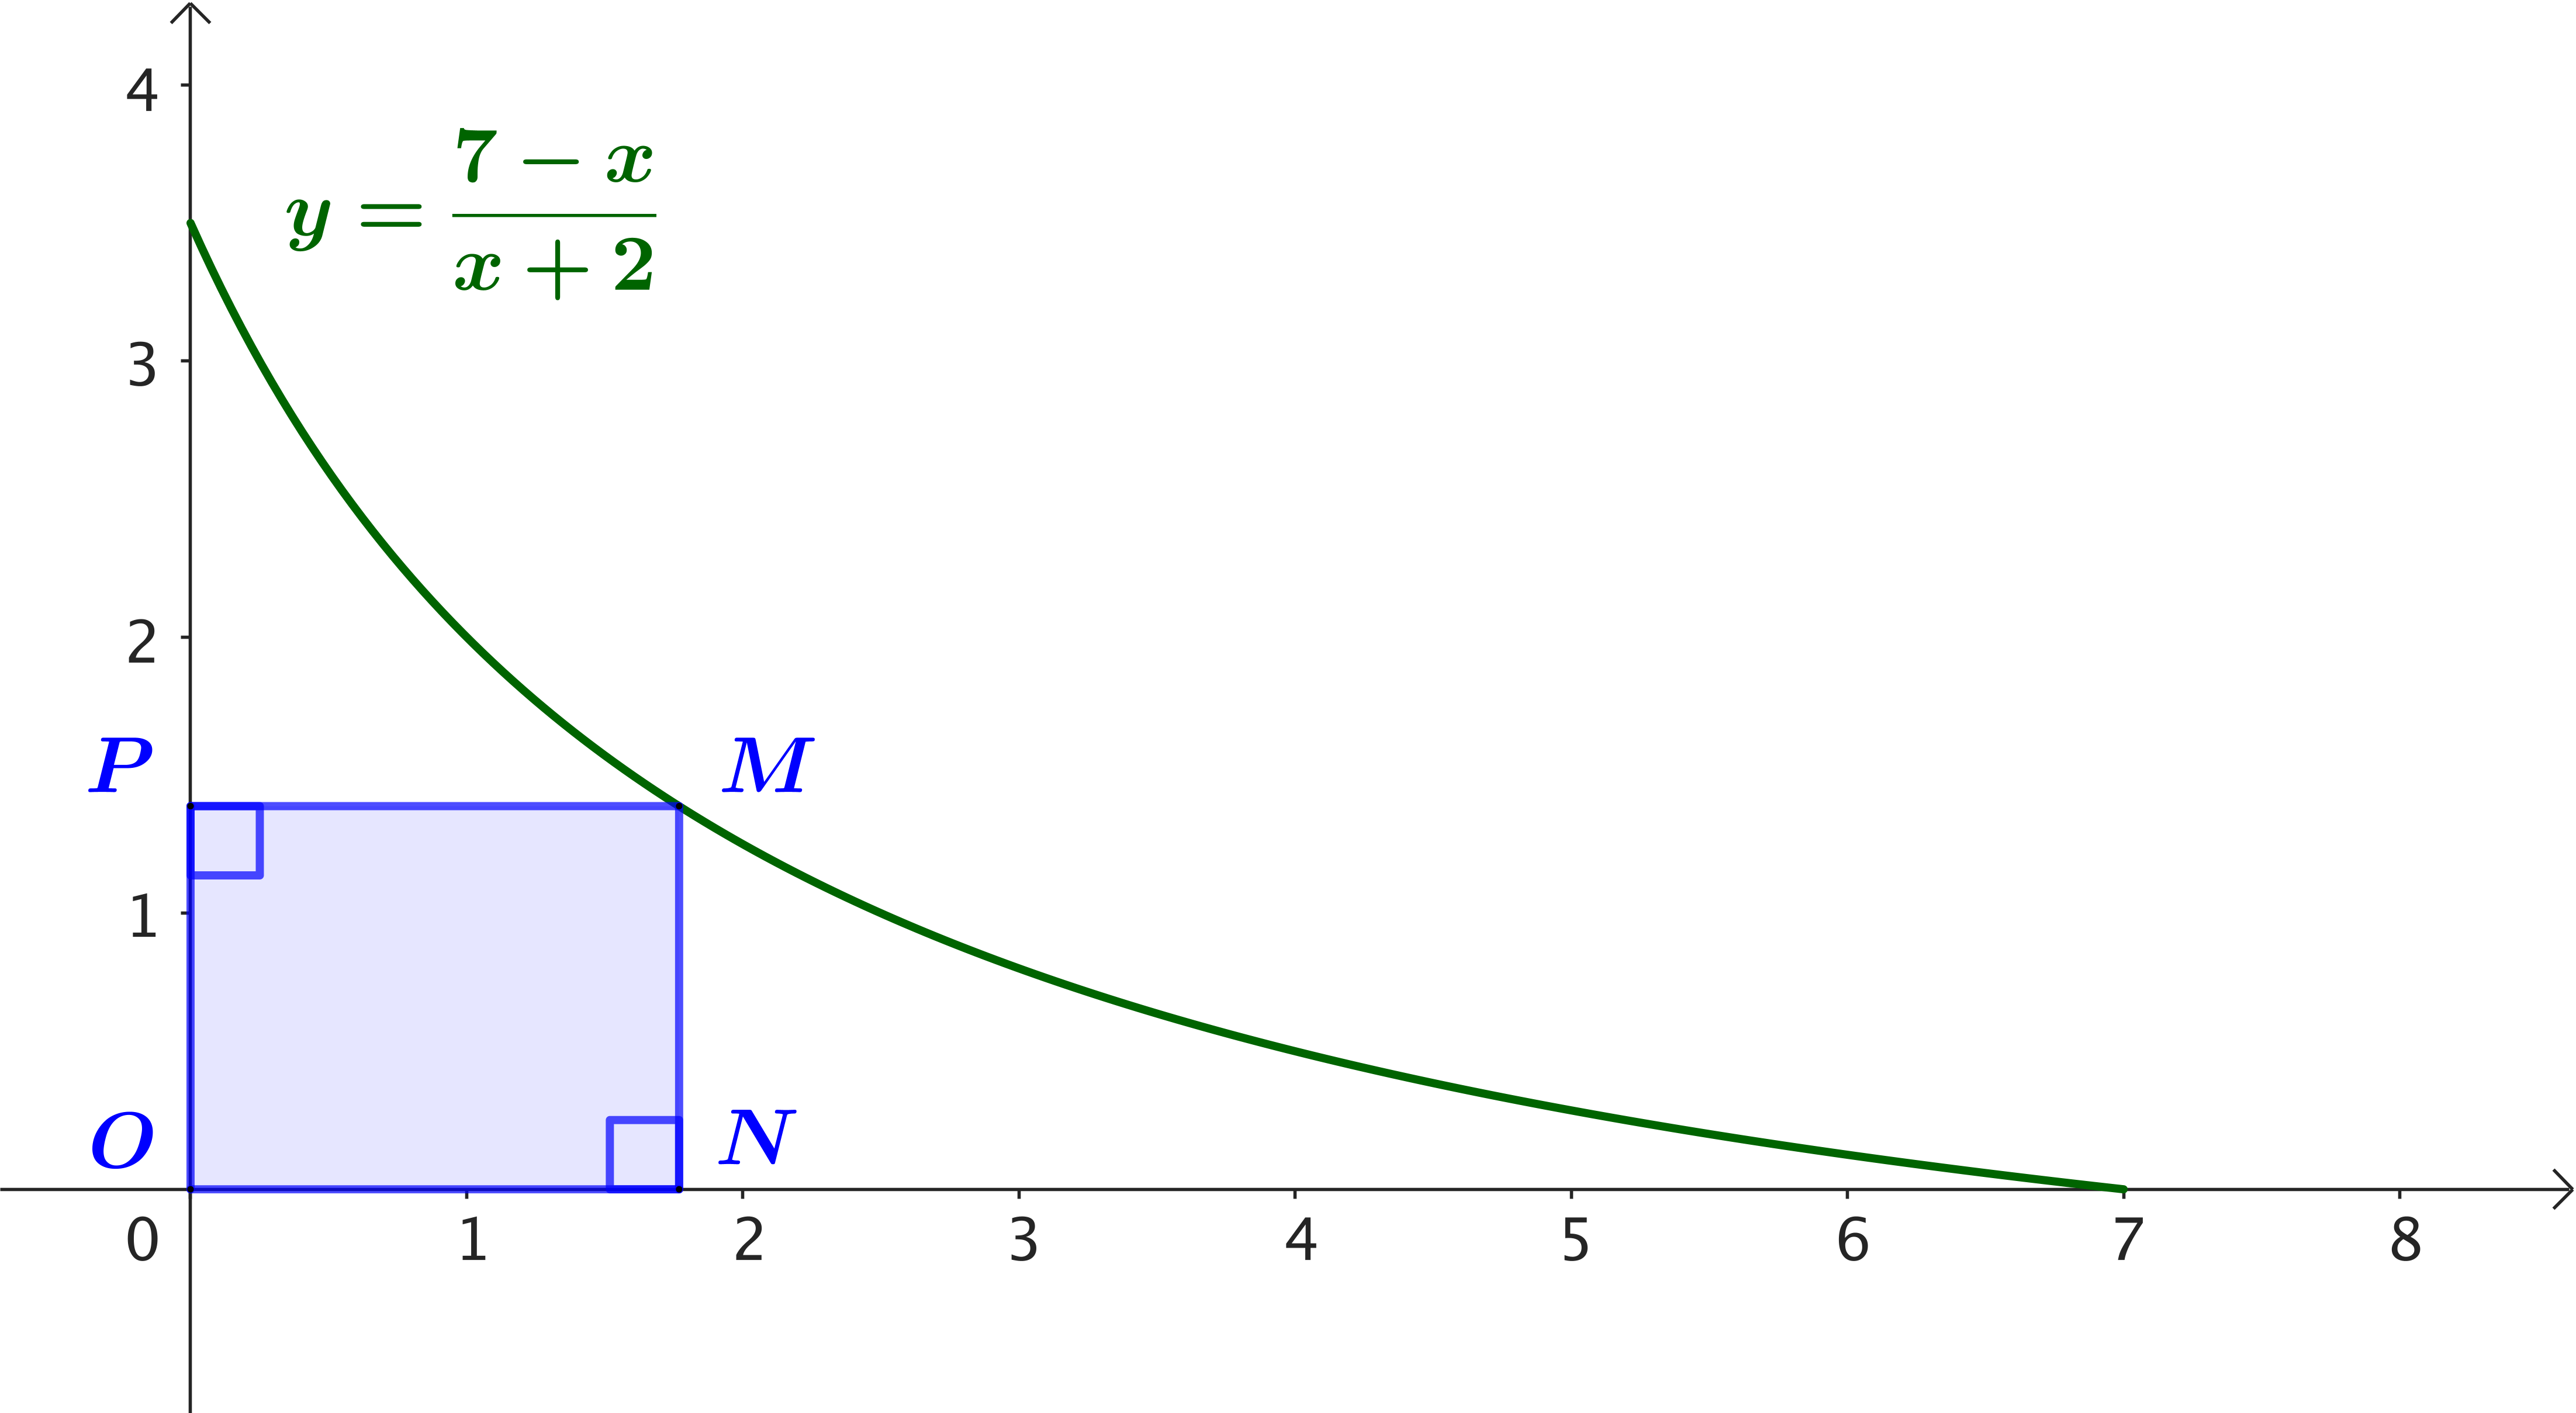
\includegraphics[scale=.67]{goal.png}
\end{center}